%please update these for each book release:

\newcommand{\bookauthor}{Noel J. Hicks}
\newcommand{\shortbookauthor}{Hicks}
\newcommand{\booktitle}{Notes on Differential Geometry}
\newcommand{\booksubtitle}{with 25 figures and 100 problems}

\newcommand{\bookcoverTeXromancers}{Revised and modernized edition by}

\newcommand{\bookcoverpicture}{
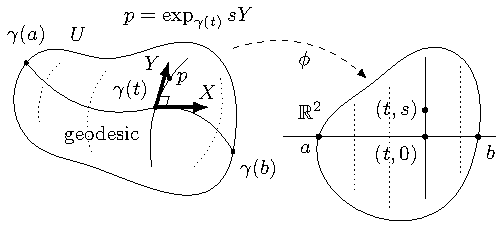
\includegraphics[height=21em]{./figure/ch9fig1_edited.pdf}
}

\newcommand{\bookoriginaledition}{1965}
\newcommand{\bookthisedition}{2022}

%these are meant for the back cover
%both should have ~100 words
\newcommand{\bookreview} 
{A concise introduction to the topics considered part of a standard background in differential geometry up until today.
\\[1em]

The first three chapters provide a crash course in classical differential geometry, leading into an intermezzo of tensors and forms, while the rest of the book introduces the notion of connexion (connection) and various topics in Riemannian geometry. The notes are intended for a full year course, covering the first six chapters in one semester.
\\[1em]

Contains a total of 100 problems of varied difficulty, consisting of computations, additional theorems and examples, results from the literature and supplementary topics such as Lie groups and bundle theory.
}

\newcommand{\bookauthorbio}
{\emph{Noel J. Hicks} (1929-1979) was born in San Antonio, Texas. His undergraduate studies took place at the University of Wyoming, and his PhD was awarded in 1957 by the Massachusetts Institute of Technology. His thesis, supervised by Warren Ambrose, was titled \emph{On the Curvature and Torsion of Affine Connexions}.
\\[1em]

After graduating, Hicks joined the University of Michigan faculty as instructor; he was appointed assistant professor in 1961, associate professor in 1966. Geometry was his field of research and advanced teaching: his textbook on differential geometry is known as a classic treatment of the subject, and he wrote a number of important research papers in the area.
}
\newcommand{\authorbiosource}{U. of Michigan, \emph{Faculty History Project}; \emph{Mathematics Genealogy Project}} %http://faculty-history.dc.umich.edu/faculty/noel-j-hicks/memorial

%\newcommand{\aboutandlegal}{} %UNUSED -- blurb about what the group is and maybe mention legal stuff in back cover